\chapter{Mini-Project B}
This project is for CS students only.\\

\section{Scenario}
Your uncle appreciates the work you have done developing a rough prototype. Because you did such a good job of developing the base system, your uncle has asked you to develop a means of a system where they can access their data remotely. You decide to do this as simply as possible, making use of an application called \href{https://blynk.io/}{Blynk}.



\subsection{Overview}
Essentially, this is a repeat of the first project, but adds a button to change the interval reading and makes the data accessible through Blynk.

\subsection{Deliverables}
At the end of this practical, you must
\begin{itemize}
    \item Submit a short write up. See the marking guide in section \ref{sec:ProjBMarks}
\end{itemize}

\subsection{Hardware Required}
The hardware from mini-project A and an additional button.

\subsubsection{Software Requirements}
\begin{itemize}
    \item You need to add Blynk.
    \item You need to add functionality for changing the reading interval between 2, 5 and 10 seconds.
\end{itemize}

\begin{multicols}{2}
Figure \ref{fig:blynkexample} shows an example of what the app you create in Blynk might look like. This is the example from last year's project, but you can see there's a terminal for accessing the output of the print statements and a space for values as read from the ADC. Last year's project also had an alarm, which is not a feature in this year's project so you need not include one. There are various widgets in Blynk. It's suggested you play with your energy budget to develop the most intuitive and aesthetically pleasing design possible.
\vfill\null
\columnbreak
\begin{figure}[H]
\centering
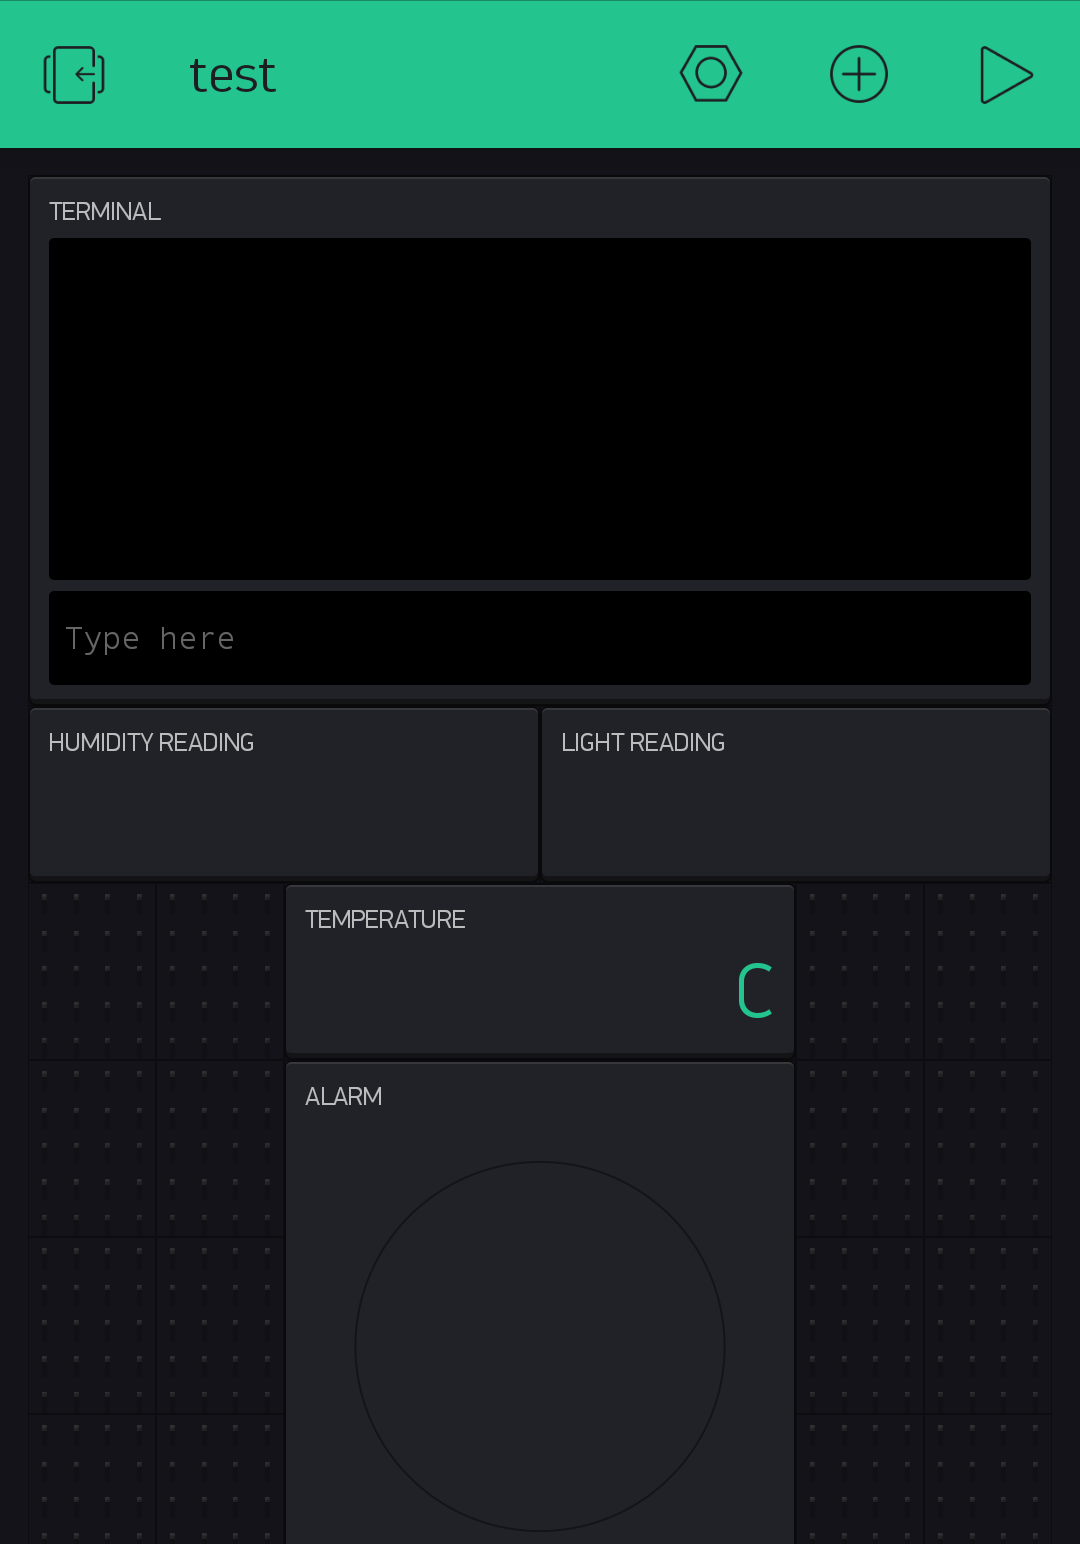
\includegraphics[width=0.75\columnwidth]{Figures/blynkexample}
\caption{Example Blynk Project}
\label{fig:blynkexample}
\end{figure}
\end{multicols}

\subsection{Marking Guide}
\label{sec:ProjBMarks}
\begin{table}[H]
\centering
\caption{The Write Up Format For mini-project B}
\label{tbl:ProjBMarks}
\begin{tabular}{|l|l|l|}
\hline
\textbf{Section of Report} & \textbf{Description} & \textbf{Marks} \\ \hline
\textbf{Introduction} & An introduction to what's new in this project & 10 \\ \hline
\textbf{Design} & \begin{tabular}[c]{@{}l@{}}Design of the system. Design of the server. \\ Talk about the stack used for development. \\ Include UML and block diagrams, and \\ mention any hardware/software\\ interfacing issues.\end{tabular} & 30 \\ \hline
\textbf{\begin{tabular}[c]{@{}l@{}}Implementation/\\ Build Proces\end{tabular}} & \begin{tabular}[c]{@{}l@{}}Some code snippets and steps in building \\ the device and server.Can think of this as a\\ simple methodology.\end{tabular} & 15 \\ \hline
\textbf{Instructions for use} & \begin{tabular}[c]{@{}l@{}}How to operate the system. You should \\ include some screenshots and photos.\end{tabular} & 15 \\ \hline
\textbf{Testing/Results} & \begin{tabular}[c]{@{}l@{}}How did you ensure your system works? \\ What did you do to test the functionality, \\ and what were the results? You can include\\ screenshots or photos, but you need to talk \\ about them (it's not enough to just have a \\ photo).\end{tabular} & 20 \\ \hline
\textbf{Conclusions} & \begin{tabular}[c]{@{}l@{}}How well did your system work? Did you \\ achieve the objectives? What could you do \\ to improve the system?\end{tabular} & 10 \\ \hline
\textbf{TOTAL} &  & \textbf{100} \\ \hline
\end{tabular}%
\end{table}


\chapter{Acknowledgements}
\begin{enumerate}
    \item Image use \href{https://onlineplantsindubai.weebly.com/uploads/1/0/9/0/109064913/air-plants-terrarium-as-bearded-dragon-terrarium_1_orig.jpg}{onlineplantsindubai.weebly.com}
    \item The meme template used in Figure \ref{ButterDragon} is of Butter the bearded dragon, which is accessible through a Google search
\end{enumerate}

\newpage

\textbf{Declaration of non-plagiarism}

\begin{itemize}
    \item I know that plagiarism is wrong. Plagiarism is to use another’s work and pretend that it is one’s own.
    \item I have used the \rule{4cm}{1pt} convention for citation and referencing. Each contribution to, and quotation in, this essay/report/project/submission from the work(s) of other people has been attributed, and has been cited and referenced.
    \item This essay/report/project/submission is my own work.

    \item I have not allowed, and will not allow, anyone to copy my work with the intention of passing it off as his or her own work. 

\end{itemize}

 

Name \rule{4cm}{1pt}  Student Number \rule{4cm}{1pt}

 

Signature \rule{4cm}{1pt}     Date \rule{4cm}{1pt}

 